\section{Giới thiệu về Android}
Như chúng ta biết, hiện tại đã có hơn nửa nhân loại sử dụng máy di động để thoại và giao tiếp qua các mạng không dây. Con số 3 tỉ người này sẽ còn tăng lên và máy di động càng ngày càng "thông minh" với nhiều chức năng và dịch vụ rất hấp dẫn, cho nên thị trường máy di động thông minh sẽ vượt xa máy vi tính trong một tương lai rất gần... Vì thế việc lập trình trên thiết bị di động ngày càng phổ biến và phát triển rất mạnh mẽ. Từ nền tảng mã nguồn mở, Google đã cho ra mắt Android chạy trên các thiết bị di động. Android có rất nhiều công cụ và dụng cụ miễn phí để nghiên cứu và phát triển phần mềm trên nền tảng của nó. Trong đồ án này, ta sẽ tìm hiểu về Android và cách viết một ứng dụng trên nền tảng này.

\subsection{Khái niệm về Android}
Trước hết, Hệ điều hành (Operating System - OS) là phần mềm hệ thống quản lý phần cứng máy tính, phần mềm và cung cấp các dịch vụ chung cho các chương trình máy tính.
Android là hệ điều hành dựa trên mã nguồn mở Linux OS cho các thiết bị di động và các thiết bị thông minh như máy tính bảng, laptop, netbook, smartbook, TV thông minh(Google TV),\dots Hiện nay, một số hệ điều hành cho thiết bị di động: Android, OS X (iPhone), Windows Mobile, Symbian,\dots Tuy nhiên, hệ điều hành được sử dụng nhiều nhất là Android và OS X.
\newline
% Điểm nổi bật của Android
Ngay từ khi ra mắt, Android đã gây ấn tượng mạnh khi đây là đứa con của Goodle sử dụng giấy phép mã nguồn mở. Android là sản phẩm kết tinh từ ý tưởng của Khối Liên minh thiết bị cầm tay mở do Google dẫn đầu, gồm 34 thành viên với các công ty hàng đầu về công nghệ và di động toàn cầu như Qualcomm, Intel, Motorola, Texas Instruments và LG Electronics, các nhà mạng như T-Mobile, Sprint Nextel, NTT DoCoMo và China Mobile.
\newline
% Đặc tính mở của Android
Với đặc tính "mở", Android cho phép các nhà phát triển có thể sử dụng miễn phí bộ Kit Android Software Development để xây dựng các ứng dụng của mình. Ví dụ, một ứng dụng có thể gọi bất kì chức năng lõi của điện thoại như thực hiện gọi, gửi tin nhắn, sử dụng máy ảnh,\dots Điều này thực sự thu hút các nhà phát triển sáng tạo ra các phần mềm hấp dẫn, từ đó tạo ra một cộng đồng phát triển lớn - là nguyên nhân đến sự phổ biến của Android như hiện nay.

\subsection{Kiến trúc của Android}
Để bắt đầu lập trình với Android, chúng ta cần nghiên cứu qua bản thân HĐH Android, chúng ta không cần hiểu quá chi tiết, nhưng trước hết là cần có cái nhìn chung và toàn diện nhất về Android.
\newline
Android Platform bao gồm đầy đủ các tính năng HĐH Android, các ứng dụng và các tâng trung gian để nhà phá triển có thể mở rộng, tùy chỉnh thêm theo nhu cầu của họ. Có 4 tầng cơ bản trong HĐH Android: Linux Kernel, Native Libraries, Android Runtime, Application Framework,\dots Các tầng làm việc có sự liên kết với nhau.
\begin{enumerate}
    \item{\textit{Tầng Linux Kernel:}}
    Đây là tầng nhân của HĐH Android, Linux Kernel giúp hệ điều hành có thể giao tiếp với phần cứng của thiết bị như: camera,  USB, Wifi, Bluetooth, Display, Power Management,\dots  Linux Kernel chịu trách nhiệm cho các trình điều khiển thiết bị, quản lý nguồn điện, quản lý bộ nhớ, quản lý thiết bị và truy cập tài nguyên. Kernel hoạt động như một lớp trừu tượng giữa phần cứng và phần mềm còn lại của hệ thống.
    \item{\textit{Native Libraries:}}
    Native Libraries là tập hợp của nhiều thư viện như WebKit, OpenGL, FreeType, SQLite, Media, SSL,\dots 
    \item{\textit{Tầng Android Runtime:}}
    Android Runtime cung cấp một thành phần quan trọng được gọi là DVM (Dalvik Virtual Machine - máy ảo) có trách nhiệm chạy ứng dụng android.
    DVM thực thi các file có định dạng .dex (Dalvik Excutable), định dạng này là định dạng được tối ưu hóa về bộ nhớ.
    \newline
    DVM có phần tương tự như JVM (Java Virtual Machine) nhưng được tối ưu hóa cho các thiết bị di động như tiêu thụ ít bộ nhớ hơn và tăng hiệu suất hoạt động tốt hơn.
    \item{\textit{Tầng Application Framework:}}
    Application Framework bao gồm tập hợp những API cho phép các nhà phát triển ứng dụng được phép sử dụng các dịch vụ này trong các ứng dụng của họ.
\end{enumerate}
Ở góc độ người dùng, ta có thêm tầng Application - là các ứng dụng do nhà phát triển ứng dụng viết. Sau đây là sơ đồ tương quan liên kết giữa các tầng:
% 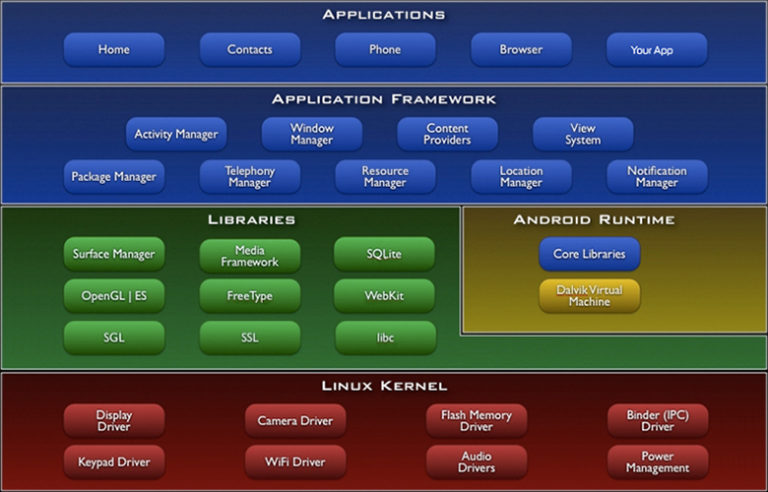
\includegraphics[]{images/android-flatform.jpg}


